%%%%%%%%%%%%%%%%%%%%%%%%%%%%%%%%%%%%%%%%%%
\chapter{Introduction} \label{sec:introduction}
%%%%%%%%%%%%%%%%%%%%%%%%%%%%%%%%%%%%%%%%%%
The thermomechanical loads on solid breeders can hinder breeders' function in producing and releasing enough amount of tritium fuel for a DT fusion power plant. The thermomechanical loads on solid breeders, etc etc etc. For a fusion power plant to produce electricity and be self-sustaining in terms of its limiting fuel. [Blanket designs of solid breeders to meet this feasibility have evolved significantly...] The feasibility depends on the the ability engineer a device that surrounds the fusion reaction, captures the ejected neutron to breed tritium, allows recovery of that tritium to attain self-sufficiency, and delivers the energy deposited in the blanket as high quality heat into a power cycle to create electricity. Blanket designs of solid breeders have evolved significantly since their introduction in the 1970s. Some features of current breeder designs will be discussed next.

In this chapter we will present some of the basics of thermonuclear fusion of hydrogen and the need to artificially breed tritium.  Then we do some of the functions of a solid breeder / the role a solid breeder plays in the fusion power plant. Then introduce the solid breeder as a concept for the blanket. In \cref{sec:intro-bed-integrity}, we will go into more of the physics and engineering behind the need for- and approaches for maintaining- temperature control in a solid breeder. Finally in \cref{sec:intro-scope-of-work}, the scope of this work will be outlined.



\section{The Basics of Nuclear Fusion and Tritium Breeding}\label{sec:fusion-basics}
The controlled, sustained thermonuclear fusion of light elements is the ultimate energy source for humanity. Fusion is an energy source that is inexhaustable (on our planetary scales), produces none of the greenhouse gases that are altering the climate of our planet in potentially devastating ways, and avoids many of the dangers of nuclear fission. But overcoming the engineering obstacles to tame the fusion reaction is the greatest technological challenge of our generation.

The most favorable fusion reaction for first generation fusion reactors involves the two hydrogen isotopes of deuterium and tritium. The deuterium-tritium (DT) reaction has a high reaction probability at the lowest ion temperature with high energy yield. Alternative fusion reactions of two deuterium atoms or a deuterium atom with helium-3 are advantageous in other regards, such as no radioactive byproducts or fuel availability, but their relatively higher ion temperature preclude them from current consideration. The DT reaction proceeds as
\begin{align}
	\mathrm{D} + \mathrm{T}&\xrightarrow{}~^4\mathrm{He}+\mathrm{n}+17.58~\text{MeV} \label{eq:dt-reaction}
\end{align}

Of the two isotopes fused, deuterium ($D$, or $^2$H) is a stable isotope and is naturally occuring in an average abundance of 0.015 mole percent in water on Earth. To demonstrate just how plentiful deuterium is as a fuel source, there is approximately 100 million billion kilograms of deuterium in the Earth's oceans. If all energy on Earth were produced from DT fusion power plants, there would be enough deuterium to outlast the lifetime of our sun. We will not run out of peak deuterium.  

Tritium ($T$, or $^3$H), however, is radioactive with a half-life of only about 12.32 years; any naturally occurring tritium decays at such a rapid pace it will never accumulate to an appreciable amount on Earth. If tritium is to be used as a fuel in a fusion power plant, it must be generated artificially. 

A method of in-situ generation of tritium in a fusion reactor is to include a so-called tritium breeding blanket that surrounds the plasma with a phase of lithium. Natural lithium will interact with neutrons as
\begin{subequations}\label{eq:lithium-t}
\begin{align}
	\mathrm{n} + ~^7\mathrm{Li} &\xrightarrow ~\mathrm{n}+\alpha + \mathrm{T} -2.47~\text{MeV}\label{eq:li7-t}\\
	\mathrm{n} + ~^6\mathrm{Li} &\xrightarrow ~ \alpha + \mathrm{T} +4.78~\text{MeV} \label{eq:li6-t}
\end{align}
\end{subequations}
where we haved used the common short-hand of $\alpha$ in place of the helium nucleus. The cross-sections of the lithium reactions are given in Fig.~\ref{fig:li-xsects}. Note the exothermic lithium-6 reaction (a neutron of any energy will incite the transmuation) and the threshold energy required of the incident neutron in the endothermic lithium-7 reaction.

\begin{figure}
	\centering
	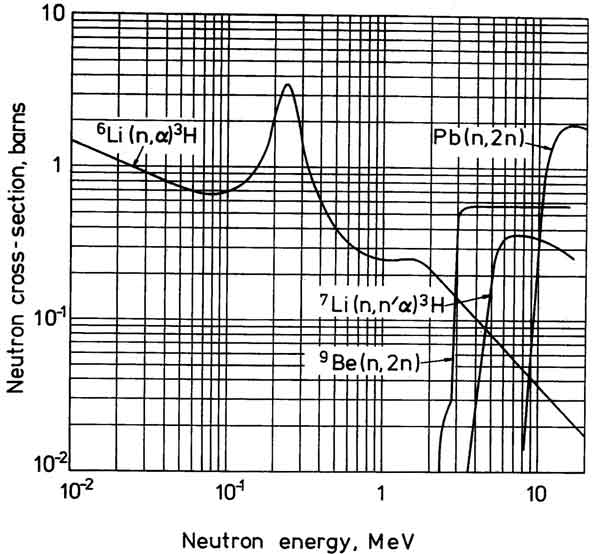
\includegraphics[width=0.75\textwidth]{chapters/figures/breeding_xsecs} 
	\caption{Cross-sections of various blanket materials. Note the threshold for the $^7$Li and neutron multiplying reactions.}
	\label{fig:li-xsects}
\end{figure}

Lithium, like deuterium, is quite abundant on Earth. As noted in Francis Chen's book on the fusion, there is enough lithium available on land to generate tritium for 30 million years of DT reactions providing all of humanity's electricity.\cite{chens-textbook}. 

To reiterate, neither the fusion reaction of Eq.~\ref{eq:dt-reaction} nor the necessary transmutations of lithium in Eqs.~\ref{eq:lithium-t} produce any greenhouse gases. The nature of fusion requires a constant supply of fuel (and extremely careful engineering) to keep the plasma burning; there is no risk of the fusion reactor going into melt-down. For even the first generation fusion reactors, the necessary fuel will last beyond the timeline of humanity on Earth. Furthermore, the next generation fusion reactors will likely move away from tritium and will have virtually no concern of radioactive waste. Fusion power is unarguably the ultimate energy source for humans on Earth and, if we continue to live the lives of comfort we currently enjoy, is in absolutely critical step in humanity's march forward.

\begin{figure}
	\centering
	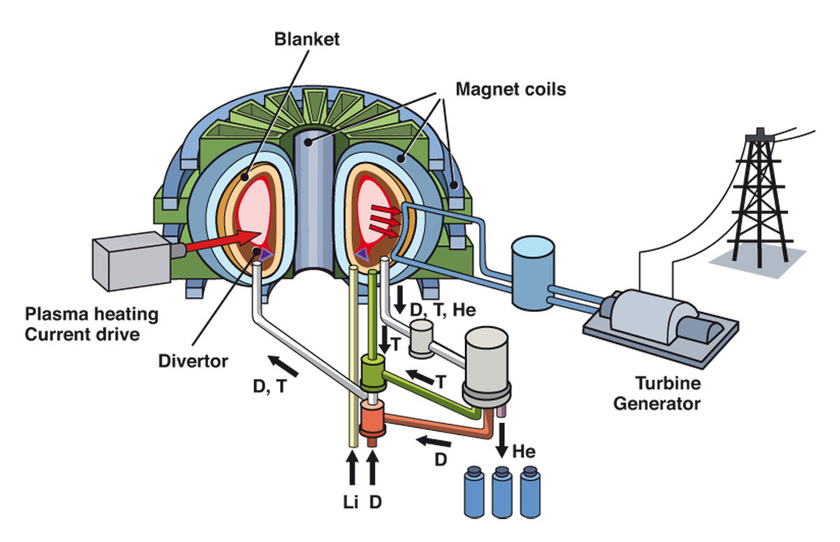
\includegraphics[width=0.85\textwidth]{chapters/figures/power-plant-schematic} 
	\caption{Schematic of a tokamak power plant showing the role of the blanket in both energy production and tritium breeding. (reproduced from the Max-Planck-Institut für Plasmaphysik)}
	\label{fig:power-plant-schematic}
\end{figure}

In Fig.~\ref{fig:li-xsects}, a schematic of a potential magnetically-confined fusion power plant is shown. In the illustration, we see the blanket surrounding the toroidally-shaped plasma and how the tritium generated in the blanket is recycled on-site to be fed back into the burning plasma. Also apparent in the sketch is the role of the breeding blanket as power generator. In \cref{sec:blanket-design}, we will go into more detail on the complete function of a breeding blanket in a fusion reactor.

%\section{The Role of Breeding Blankets}
As was shown in \cref{sec:fusion-basics}, the blanket surrounding the plasma must perform the critical role of breeding tritium from lithium. The measure of a blanket design's effectiveness at breeding tritium is commonly done with the metric of the tritium breeding ratio (TBR). The TBR is defined as the number of tritium atoms produced in the blanket per fusion neutron. When the fusion neutron is ejected it may stream through gaps in the blanket that are necessary for instrementation, plasma heating, etc. The neutron may also collide with supporting structure or other elements in the breeding material. Due to the neutron leakage and parasitic interactions, only 60-80\% of the fusion neutrons may react with lithium. Futhermore, once tritium is actually generated, it is retained in structural material or lost to the fuel cycle simply from inefficiencies in handling. It becomes quickly obvious self-sufficiency of the fuel cycle is clearly not possible unless we produce more than one tritium per fusion neutron [maybe not accurate -- check Abdou's notes]. 

One scheme for increasing the TBR of breeder blankets is to introduce beryllium as a neutron multiplier. Beryllium has a very high nuclide density while also being very light, with a high melting temperature, and has a high thermal conductivity. The incident neutron smashes beryllium into two $\alpha$ particles and an additional two neutrons. Therefore, in order to breed tritium, the blanket will first generate more neutrons for every neutron spit out by the fusion reaction.

% In addition to breeding tritium, the blanket will be responsible for power extraction in the fusion reactor. The blanket must function to capture the kinetic energy of neutrons (80\% of the fusion energy is carried by the neutron), secondary $\gamma$ rays, and the plasma radiation on the plasma-facing first wall (an integral component to the blanket). The blanket must also be able to convert the fusion's energy into high quality heat that can be extracted into the power cycle connected to the fusion reactor. 

% Finally, the last function of the breeding blanket is to provide radiation shielding of the vacuum vessel and super-conducting magnets that are containing the plasma. 

[From Alice:]there are two lines of blanket concepts using different forms of breeder: liquid or solid. In this thesis, the research is on the solid breeder blankets, specifically the blanket uses lithium ceramic breeder pebbles, as the form of solid breeder, for tritium fuel production. 
\section{Pebble bed Solid Breeder Blanket Concepts}\label{sec:blanket-design}

Material and Form
As each individual tritium breeding region is small, in a typical solid breeder blanket design there are several alternating layers of breeding zone, cooling plate, and neutron multiplier. 

[Alice suggestion:] Don't have such a long intro here. Get to the point and have some drawings to demonstrate.``You need solid breeder blanket design pictures here to help people to understand the issues/problems.''


TBM unit design

In typical solid breeder modules, coolant fluid runs through the containing structure surrounding the pebble bed. A low-pressure, low-speed purge gas is pumped through the pebble bed to extract the tritium generated and transport it out of the blanket for processing. As nuclear energy is deposited into the poorly-conductive ceramic breeder material, the temperature climbs well above the containing structure. Heat is removed from the pebble bed predominately through inter-particle conduction (with a small contribution from convection of the purge gas) and contact conductance of many pebbles pressed against the containing surface. 

The packed bed will be contained in a structure of ferritic or austenitic steel. The energy of the packed bed is carried away by coolant channels in the structure that have flowing in them high pressure helium gas. Because the structural material is held cooler than the breeding zone, it will confine the thermal expansion of the lithium ceramic and lead to mechanical stresses at the points of contact of the individual pebbles in the packed bed. Engineering design issues surrounding this thermal stress is of great concern to researchers and will be the focus of much of this report.

Once in operation, the ceramic pebble beds will have a specified operating temperature window that is dictated by tritium release characteristics. The low end of the temperature window is governed by a minimum temperature for acceptable release rates of tritium from the ceramic to the purge gas; the value is generally set around 300~\celsius. The upper limit of the temperature window is chosen to avoid sintering of the lithiated ceramic. Sintering of the ceramics, as grains in individual pebbles meld, is predicted to reduce the rate of tritium release. The upper end of the temperature window is generally set around 900~\celsius.

The size of breeder regions is limited by the temperature window combined with the poor effective conductivity of packed beds of ceramic pebbles. The conductivity is a weak function of external pressure but can generally be approximated as about \si{1 W/{mK}}. Because the effective conductivity and packed bed-wall interface conductance is predominately a contact conduction, disruptions to the packing structure will have considerable impact on the heat transfer of the packed bed.

The fusion reaction deposits a great deal of surface radiation on the first wall of the breeding blanket and the blanket will be absorbing energy deposited from neutron interactions and $\gamma$ rays. The blanket must be capable of converting and then recovering the energy at high tempreatures for efficient power production in the fusion power plant. The nuclear heat generated in the pebble bed solid breeder will heat the ceramic pebbles to maximum temperatures of approximately 900~\celsius. The heat of the pebbles is transported through them via conduction through inter-particle contacts, conduction through the purge gas into neighboring particles, and ultimately through contact with the containing structure. The box structure surrounding the solid breeder will have high pressure (\si{8~MPa} in many current designs) helium flowing through channels that remove the heat from the blanket, with the helium reaching temperatures of 500~\celsius, and into a power generation cycle.
\section{Pebble Bed Integrity, Thermophysics, and the Role of Modeling}\label{sec:intro-bed-integrity}

The pebble bed will experience a constrained thermal expansion as the hot ceramic pebbles press against the relatively cooler container. The restricted thermal expansion of the pebble bed causes an external pressure on the pebble bed. The external pressure may lead to a number of phenomena that disrupt the initial packing -- and by extension the initial predictions of thermal and mechanical properties -- of the pebble bed. For one, in experiments of even well-packed ensembles of pebbles, the beds show an apparent plastic strain of rearranged packing that increases with maximum historical stress on the bed.[cite Chunbo and Reimanns experimental papers] Without careful engineering and packing of the virgin pebble beds, plastic strain in the pebble bed will directly lead to the formation of gaps between the pebble bed and containing structure. Depending on the configuration of the solid breeder design, the gap could cause a tremendous loss of heat transport from the pebble bed to the coolant. Furthermore, any gaps formed in the blanket could lead to more neutron leakage and decreased tritium breeding ratios and detriment to the blanket's shielding function.

Additionally, assuming that the plastic strain is removed from the pebble bed, the thermally-induced pressure on the pebble bed will be balanced by the individual pebbles pressing into each other at small points of contact. The small area over which the contact forces are applied leads to stresses which may crush individual pebbles in the ensemble. With the potential accumulation of many cracked/crushed individual pebbles, the overall packing structure is again altered. Depending on the extent of crushing, the response of the pebble bed may be as benevolent as a negligible decrease in effective thermal conductivity or malevolent as a loss of physical contact and heat transport from the pebble bed to the coolant. 

Finally there are long-term effects expected in the materials experiencing prolonged exposure to cycling irradiation, heat, and stress. Thermal ratcheting, swelling, sintering, or thermally-induced creep can lead to evolutions in thermophysical properties even in the absence of cracked pebbles. As the thermophysical properties evolve, global or local bed temperatures change and ultimately the tritium release characteristics of the bed deviate from any prediction one may have had from the initial packing of the ceramic pebble bed. 

In our group we are most focused on maintaining tritium breeding characteristics of the pebble bed at desirable levels and thus maintaing temperatures in the breeding region. Alleviating any of the issues that may plague the ceramic breeder all boil down to requiring temperature control via an understanding and of the morphological changes of the ceramic packed beds and their interaction with the interstitial purge gas and structural container. [say how temperature control is possible with better models]In this work we introduce enhancements and new elements to build upon the understanding from ceramic breeder models of past research efforts. 







% Control of the manufacturing processes of the ceramic pebbles permits manufactureres to custom vary characteristics, such as the pebble's:
% \begin{itemize}
% \item tritium retention and release properties.
% \item Lithium density
% \item Opened- and closed-porosity
% \item Nominal diameter
% \item and, indirectly, crush strength. 
% \end{itemize}
% However the characteristics of the pebble are often coupled. For instance, for the sake of tritium management the open porosity of the pebble is often increased. But this comes at the expense of a decreased crush strength of the pebble. Because of the relatively weak crush strength distributions among batches of pebbles as well as the value of stresses predicted in the pebble bed, it is inevitable that during operation in the fusion environment individual pebbles will `fail' in the ensemble. Designers of lithium ceramic tritium breeding blankets must mitigate pebble failure but also anticipate the breadth and magnitude of effects that some unavoidable failure will have on macroscopic properties.



% [EDIT: THIS PARAGRAPH IS NOT NECESSARY? I DON'T NEED TO MAKE THE CASE FOR USING DEM. I JUST NEED TO EXPLAIN THE MODEL]The volume of a pebble in a tritium breeder is on the scale of 10$^{-9}$~m$^3$ while the typical container volume can be on the order of 10$^{-2}$~m$^3$\cite{Cho2008}.  Thus a single breeder volume will house upwards of $N = 10^7$ pebbles. Statistically then, the behavior of any single pebble seems insignificant and instead the entire ensemble of pebbles may be treated as a continuous media. Continuum theory for the is the basis of finite element method models that have been able to predict thermomechanical behavior with reasonable accuracy\cite{DiMaio20081287,Zaccari20081282,Gan:2009vn}. However, after the pebble beds are placed into the fusion environment they will be required to operate for long duty times without maintenance. Thus, as time progresses the accumulation of individual failed pebbles will eventually have consequences for the macroscopic thermomechanics.  and no continuum theory exists to account for this. Instead, we turn to the discrete element method to provide a solutino.

\section{Scope of the work}\label{sec:intro-scope-of-work}
[Here we need an objective (or objectives) first. Perhaps you mention the objective in the middle of the section. It should be clearly written in the beginning of the section-- The objective of this research is to create modeling tools to be able to simulate the pebble bed morphology evolution, and to address consequent heat transfer and temperature, and to provide ----. 

scope of work- 1. to develop a transient DEM code for simulating pebbled bed morphology evolution, 2. to develop DEM coupled CFD code for heat transfer and temperature analysis, 3. to assess thermal mixing using LBM, 4. to apply the developed modeling tools for blanket pebble bed design thermal evaluations, 5. further implication---.]




To develop a complete numerical model for a pebble bed requires completing many interacting sub-models. To demonstrate, we give here the path of a possible analysis scheme of these models. To begin, one must have knowledge of the interaction of the pebble bed with the containing structure as they exist in a fusion environment. The interactions are generally analyzed via the finite element method to find internal stresses and temperature fields of the entirety of the pebble bed and surrounding container. After the internal fields are mapped into the bed, one would use the discrete element method (DEM) to interpret the macroscopic stress fields into the inter-particle forces. With the inter-particle forces and total absorbed thermal energy calculated, a prediction of the initiation and evolution of morphological changes (i.e. crushed pebbles, sintering, creep, etc.) to each computational volume. Following this, DEM would calculate new effective properties as a result of the morphological changes to the pebble bed region. Finally, the updated bed properties would feed back into the FEM formulation to update calculations in the macroscopic stress fields. A suite of integrated numerical tools that follows this example algorithm is the goal of the Fusion Science and Technology Center at UCLA, but we are far from that at this time. The work of this dissertation is focused entirely on the development of pebble-scale simulations that are predominately in the realm of the discrete element method.

We aim to provide designers of packed beds with tools to understand how packing states may evolve from time-dependent phenomena (e.g. sintering, creep, pebble cracking, etc.). These phenomena may, for instance: decrease the effective thermal conductivity which will raise bed temperatures beyond initial predictions, produce isolated pebbles which will sinter and potentially decrease tritium release rates, or even form gaps between pebble beds and containing structures leading to divergence from properties of the initial packing of the bed.

Modeling research on ceramic pebble beds should have as its main objective a thorough understanding of the evolution of pebble bed morphology and the impact on thermo-physical properties; allowing for temperature control of breeder pebble beds over the entire lifetime of the blanket. To accomplish that goal, this current study is aimed at developing a methodology for coupling established discrete element models of individual pebbles in the ensemble with thermo-fluid simulations of the interstitial helium purge gas. Specifically, we will address the impact of helium on the thermal transport in a bed experiencing evolving morphology due to cracked pebbles.

Specifically, much of the work in this dissertation concerns the evolution of thermo-physical properties of a pebble bed in the presence of crushed individual pebbles. When a pebble in an ensemble is crushed or cracked it loses contact with its neighboring pebbles and subsequently breaks any thermal or mechanical transport that the pebble was providing -- ultimately this is manifest in measurable changes to thermo-physical properties. We attempt to quantify the evolving thermo-physical changes with increasingly sophisticated DEM models of ceramic pebble beds.


%DEM
\subsection*{DEM}
In the first study of \cref{sec:dem-studies}, we analyze the effective thermal conductivity of a pebble bed assuming different fractions of pebbles in the ensemble are completely crushed. The focus of this study is to determine the extent of change in aggregate ensemble properties due to individual pebble crushing, relate the changes in effective conductivity to quantifiable pebble-scale properties (e.g. contact force, coordination number, etc.), as well as help designers anticipate acceptable limits of pebble loss from a thermal management point of view. For the DEM tools used in this study, the only mode of heat transfer is conduction between the solid particles. 



%CFD-DEM
\subsection*{CFD-DEM}
In a fusion breeder, the helium purge gas winding through the interstitial gaps of the pebbles has a substantial contribution to overall heat transfer.\cite{Reimann:2002mi,Abou-Sena2005} The model of \cref{sec:dem-studies} is improved to include the flowing interstitial gas. In \cref{sec:cfd-dem-studies}, we continue to employ our DEM tools to provide particle-scale information such as contact force, but couple the pebbles to a volume-averaged computational fluid dynamics (CFD) code. The coupled CFD-DEM model is again used to simulate the heat transfer in packed beds of ceramic spheres that experience pebble crushing -- but now investigate the impact of a flowing interstitial helium purge gas when pebbles are crushed.



%APPLICATION -- ORIENTATION OF CONTAINER
\subsection*{Applied CFD-DEM}
In the study of \cref{sec:applied-studies}, we apply our coupled CFD-DEM computational tools to the analysis of ITER-relevant solid breeder geometries. In this study we consider the combined effects of pebble crushing, packing restructuring due to both gravity and the unbalanced force network in the pebble bed, and convection from helium purge gas on temperature profiles in solid breeders for different breeding configurations. In typical solid breeder modules, coolant fluid runs through the containing structure surrounding the pebble bed. Heat is removed from the pebble bed predominately through inter-particle conduction and contact conductance of many pebbles pressed against the containing surface. As such, heat transfer out of the pebble bed relies on maintaining good pebble-pebble and pebble-wall contact. However, physical contact is interrupted to different degrees when a pebble bed responds to various amounts of individual crushed pebbles. Furthermore, the restructuring of the pebble bed after a pebble crushing event is, in part, dependent on gravity forces acting upon each pebble in the ensemble. We investigate two representative pebble bed configurations where heat is removed from the bed via inter-particle conduction, convection of purge gas, and contact between the pebble bed and its container. In the first, the coolant containing structural walls (heat transfer walls) are oriented parallel to the gravity vector. In the second configuration, the heat transfer walls are perpendicular to the direction of gravity. To simulate a crushed pebble, we replace the pebble with many smaller, non-cohesive elements while maintaining mass-conservation between the original solid pebble and crushed fragments. The fragments are then free to resettle into interstitial gaps and the rest of the bed resettles as determined by forces from gravity, contact of neighboring particles, and even the small influence of the moving purge gas. The thermo-fluid interaction with the helium purge gas will be included with volume-averaged Navier-Stokes and energy equations. The representative solid breeder volumes will be compared with respect to their temperature peaks and profiles and how those temperatures vary as a function of the percentage of crushed pebbles in the ensemble. The results can be used to optimize solid breeder pebble bed designs through the choice of breeding zone orientation relative to the gravity vector.


%LBM
\subsection*{LBM}
The models used to account for helium purge gas in the studies of \cref{sec:cfd-dem-studies,sec:applied-studies} assume effective drag or heat transfer coefficients for pebbles in a computational volume and then include the pebble influence through effective source/sink terms in the momentum and energy equations. The volume-averaged approach allows for simpler meshing of the fluid volume while still retaining much of the physical realism of the system. Complete models of the conjugate heat transfer of both the fluid moving through the tortuous interstitial gaps pebble beds pressing each other with small contact areas are intractable with current computational hardware and finite-element modeling techniques. To overcome deficiencies in computational power, in \cref{sec:modeling-lbm}, we apply the lattice-Boltzmann algorithm to our pebble bed with helium. The lattice-Boltzmann method (LBM) is a non-traditional fluid simulation technique that allows us to resolve pebble-scale interactions with bed-scale conjugate heat transfer with flowing gas on realistic simulation time scales. The LBM approach is applied to the same pebble beds analyzed in \cref{sec:cfd-dem-studies} to provide comparison between the two modeling techniques. Furthermore the LBM model, accounting for the complex helium purge gas pathways, provides more insight to the influence of helium on the heat transfer in the heat transfer of packed beds.


%Background studies
% \subsection*{Other kinds of studies and shit}
% \cref{sec:studies-experiments}
% \cref{sec:studies-numerics}












In Part II (\cref{sec:hertz-theory,sec:modeling-heat-transfer,sec:modeling-pressure-drop}) we survey the state of the art in analysis of ceramic pebble beds, contact mechanics, and modeling thermal and mechanical interactions of packed beds.  In Part III (\cref{sec:modeling-dem,sec:modeling-cfd-dem,sec:modeling-lbm}) we outline the numerical methodology of the models and tools used in this study, namely: the discrete element method (DEM), coupled computational fluid dynamics and the discrete element method (CFD-DEM), and an integrated lattice-Boltzmann method (LBM). We employ our physics knowledge and numerical tools to cover a range of studies in Part IV (\cref{sec:cfd-dem-studies,sec:dem-studies,sec:lbm-studies,sec:studies-experiments}). Finally, in Part V, we discuss the future of the current work and any limitations or interesting work that was beyond the scope of this dissertation.